\documentclass[11pt]{article}
\usepackage[margin=1in]{geometry}
\usepackage{booktabs}
\usepackage{array}
\usepackage{amsmath,amssymb}
\usepackage{xcolor}
\usepackage{graphicx}
\usepackage{caption}
\usepackage{tikz}
\usetikzlibrary{shapes.geometric,arrows.meta,positioning,calc}
\usepackage[colorlinks=true,linkcolor=blue,urlcolor=blue,citecolor=blue]{hyperref}
\usepackage{titlesec}
\titlespacing*{\section}{0pt}{1.4ex}{0.8ex}
\titlespacing*{\subsection}{0pt}{1.1ex}{0.5ex}
\setlength{\parskip}{0.4ex}
\newcommand{\x}{$\times$}
\definecolor{live}{RGB}{45,106,79}
\definecolor{dead}{RGB}{157,2,8}
\definecolor{killc}{RGB}{108,117,125}
\definecolor{pendc}{RGB}{214,104,0}
\newcommand{\pend}[1]{\textcolor{pendc}{\textbf{[#1]}}}

\title{\vspace{-3em}\textbf{Phantom Headroom: How Much Prefetch Gain in Caching\\ Survives an Honest Ruler, and Why What Survives\\ Cannot Be Captured}}
\author{}
\date{Draft v2, July 2026}

\begin{document}
\maketitle
\vspace{-3em}

\begin{abstract}
\noindent Learned and oracle-guided prefetchers are credited with large cache hit-rate gains, but those gains are typically measured against under-tuned baselines, at unmatched prefetch bandwidth, and against clairvoyant ceilings that conflate hits a deployable policy could reach with hits it never could. This paper contributes an honest ruler, a verdict, and a mechanism. The ruler is a pre-registered, bandwidth-matched instrument that isolates the \emph{learnable} prefetch headroom of a workload: the baseline is tuned adversarially (Markov-1/2/3 and an LSTM, fully swept under an explicit traffic cap), the clairvoyant ceiling receives exactly the baseline's prefetch byte budget, and the ceiling is restricted to objects inside the predictor's training vocabulary so that compulsory-miss elimination, reachable only by an oracle, is priced out at equal budget. Across 12 production traces spanning CDN, key-value, and block storage, gross corridors of $+10$ to $+33$ hit-rate points deflate by 14--87\%; genuine learnable headroom survives on 3 of 12 traces, measuring $+12.7$ to $+19.7$ points with bootstrap confidence intervals clear of a pre-registered bar. The verdict concerns those survivors: a ladder of pre-registered oracle decompositions, each isolating one ingredient of a hypothetical learned scheduler, shows that reinforcement-learned arbitration adds under one point, that fetching at prediction time captures at most 6\% of the corridor even with a perfect forecaster, and that causal insertion timing, the one remaining ingredient, misses its window on the overwhelming majority of fetches. The corridor is real but priced in clairvoyance. The mechanism is \emph{endogenous slack}: a policy's own mistimed fetch volume destroys the cache-residence window its timing model depends on, so rank-level lag learnability (which a standard gate certifies) never converts into placement-level accuracy (which insertion requires). Ported to LLM KV-cache serving on production traces, the same instrument returns a third distinct verdict: no corridor exists at all, because a tuned association table already sits on the physically reachable ceiling. Three workload families, three different pre-registered reasons not to build a learned scheduler, each reached before a single model was trained. The instrument, the ladder, and all replay code are released.
\end{abstract}

\section{Introduction}
A cache prefetcher is judged by the hits it adds. The literature's customary yardsticks for how many hits \emph{remain addable} are generous ones: the gap to Belady's clairvoyant optimum~\cite{belady}, the gap to an oracle prefetcher, or the gap over LRU. Each yardstick inflates in its own way. Belady's bound ignores prefetching entirely, and its prefetch-aware repair (Demand-MIN~\cite{demandmin}) shows the ``optimum'' itself moves once prefetching enters. Oracle-prefetcher ceilings silently spend whatever bandwidth they like, while the baselines they are compared to are throttled or simply under-tuned. And clairvoyant ceilings eliminate \emph{compulsory} misses, first requests to objects never seen before, which no deployable, history-based policy can prefetch at all.

The field's default response to an impressive headroom number is to build a learned system that chases it. This paper takes the opposite route and argues it is the scientifically prior one: first construct a ruler that cannot flatter, then ask, with pre-registered oracle experiments rather than trained models, whether the headroom the ruler certifies is capturable by any causal policy at all. Both steps produce publishable surprises. The ruler deflates most celebrated headroom into measurement artifact. The capture analysis then shows that even the honestly measured remainder is unreachable: every ingredient a learned scheduler could contribute is priced, one oracle at a time, and the binding ingredient turns out to be one no causal model can supply.

The project's own history is part of the evidence. The first measurement of ``timing headroom'' on a synthetic workload showed a corridor of $+42$ points between a tuned baseline and an oracle. All of it evaporated under two corrections (tuning the baseline's predictor family instead of only its thresholds, and granting the oracle exactly the baseline's prefetch byte rate), landing at $-0.02$. Each subsequent hardening of the protocol converted another celebrated number into an artifact; Section~\ref{sec:audit} gives the audit trail, including retractions of this project's own intermediate results. The discipline that survived, pre-registered gates, machine-checked invariants, and oracle decompositions that must kill something to be trusted, is presented here as a portable method, not an anecdote.

\paragraph{Part I: the instrument (\S\ref{sec:instrument}--\S\ref{sec:substitutes}).} A pre-registered, iso-bandwidth measurement whose central object is the \textbf{learnable corridor}: the gap between an adversarially tuned baseline and a clairvoyant ceiling restricted to objects the baseline's predictor could ever have learned, at the baseline's exact prefetch byte budget. On 12 production traces, gross corridors deflate 14--87\%; three traces retain corridors of $+12.7$ to $+19.7$ points with bootstrap confidence intervals clear of the pre-registered 8-point bar. A $2\times2$ interaction study ($n{=}6$) finds eviction quality and prefetching are \emph{substitutes}, not complements, an argument against joint eviction-plus-prefetch co-training.

\paragraph{Part II: the capture ladder (\S\ref{sec:ladder}).} Given a certified corridor, can any deployable policy capture it? The \textbf{Necessity Ladder} answers with a sequence of pre-registered gates, each an oracle decomposition that isolates exactly one ingredient and prices it by replay before any model is trained. The results, on both live traces:
\begin{itemize}\itemsep0.1em
\item \textbf{Arbitration does not need learning.} A non-separable (knapsack) dispatcher beats a threshold rule by under one point everywhere: reinforcement learning for prefetch arbitration is measurably unnecessary here (\S\ref{sec:f4}).
\item \textbf{Perfect timing of the offered stream loses.} A clairvoyant scheduler applied to the candidates the tuned predictor actually emits lands \emph{below} the baseline: the corridor is not a timing-of-what-is-offered problem but a coverage problem (\S\ref{sec:f1stream}).
\item \textbf{Coverage plus clairvoyant timing reaches the corridor.} Widening the emission fanout and inserting each object just in time recovers the corridor on both traces, so the headroom is reachable in principle (\S\ref{sec:f5}).
\item \textbf{Fetching at prediction time captures $\leq$6\% of that ceiling, even with a perfect forecaster.} Holding wide-net fetches from emission until use thrashes the cache; just-in-time insertion is isolated, cleanly, as the one missing ingredient (\S\ref{sec:policy1}).
\item \textbf{Causal insertion timing fails.} A hazard model of time-to-next-use, though it passes the standard rank-learnability gate, cannot place insertions: fetches are LATE-dominated at every hedging quantile \pend{final F7 capture and CI pending; primary runs completing}(\S\ref{sec:f7}).
\end{itemize}
The mechanism (\S\ref{sec:slack}) is named \textbf{endogenous slack}: the residence window a timing model must hit is not a property of the workload but of the policy's own fetch volume, and it shrinks exactly when the model mistimes. This explains why rank-learnability of reuse lags (Spearman $\rho\approx0.6$) coexists with placement failure, a distinction between \emph{learnable} and \emph{actionable} that headroom studies do not currently draw.

\paragraph{Part III: the ruler in a second domain (\S\ref{sec:llm}).} Ported to LLM KV-cache serving on production traces from a large deployed system, with two domain-honest adaptations (warming is decided at request boundaries, and the reachability restriction becomes physical: a KV block never computed and stored cannot be warmed by any system), the instrument returns a third verdict: \emph{no corridor exists}. A tuned association table already sits within noise of the physically reachable, bandwidth-matched clairvoyant ceiling on both traces. Three workload families now carry three distinct, pre-registered verdicts, each reached before training a model: corridor absent (block storage), corridor present but clairvoyance-priced (CDN/KV), corridor absent because the trivial policy is already optimal (LLM serving).

\paragraph{Contributions.}
\begin{itemize}\itemsep0.1em
\item A pre-registered, iso-bandwidth instrument for prefetch headroom whose central object is the \textbf{learnable corridor}, with machine-checkable invariants and a taxonomy of four corridor-inflation mechanisms, each caught by a named component (\S\ref{sec:instrument}--\S\ref{sec:audit}).
\item A deflationary measurement across 12 production traces: 14--87\% of gross corridors are phantom; 3 of 12 traces retain learnable headroom, bootstrap-confirmed; eviction and prefetching are substitutes ($n{=}6$).
\item The \textbf{Necessity Ladder}: a method for pricing each ingredient of a hypothetical learned scheduler by pre-registered oracle decomposition before training, and its verdict here, a triple kill (learned arbitration unnecessary, at-emission dispatch insufficient, causal timing unreachable) that converts the surviving corridor into a \emph{clairvoyance-priced} quantity.
\item The \textbf{endogenous slack} mechanism, separating rank-learnability from placement accuracy, with direct measurement of both.
\item The first honest headroom measurement for \textbf{LLM KV-cache warming}, showing a tuned table already sits on the physical ceiling of Mooncake production traces, and with it a three-domain demonstration that the instrument discriminates rather than merely deflates.
\end{itemize}
No prevalence claim is made (``most workloads have headroom'' is exactly the kind of claim this instrument exists to prevent). The claims are existence with confidence intervals, absence with mechanisms, unreachability by oracle decomposition, and a protocol that lets anyone locate their own workload on the map.

\section{Related Work}
\paragraph{Optimal replacement and its prefetch-aware repairs.} Belady's MIN~\cite{belady} is optimal for demand caching without prefetching. Jain and Lin's Demand-MIN~\cite{demandmin} showed that under prefetching, MIN no longer minimizes demand misses and that a family of prefetch-aware optima trades demand misses against prefetch traffic, establishing, for hardware caches with uniform lines, that ``the optimum'' is bandwidth-relative. The instrument here transports that insight to variable-size object caches and adds the reachability split: it bounds not what an omniscient policy could do but what a history-based one could. Cao, Felten, Karlin and Li~\cite{cao} gave near-optimal integrated prefetching-plus-caching under clairvoyance, uniform sizes, and a fetch-latency model; none of the three assumptions holds for CDN/KV objects, which is why ceilings are measured empirically per trace instead of cited as guarantees.

\paragraph{Learned caching systems.} Learning Relaxed Belady (LRB)~\cite{lrb} imitates a relaxed Belady oracle for CDN eviction; Cold-RL~\cite{coldrl} learns eviction for NGINX via offline RL; DEAP~\cite{deap} learns admission, eviction and prefetching jointly with supervised sequence models; DeePref~\cite{deepref} learns prefetching for video CDNs online; LightCacheRL~\cite{lightcache} unifies prefetch and replacement decisions in a myopic bandit; Pythia~\cite{pythia} tunes hardware-prefetcher aggressiveness with online RL and bandwidth feedback; and Yuan et al.~\cite{jointhw} share representations between hardware replacement and prefetching policies. \textbf{Baleen}~\cite{baleen} is the nearest neighbor: it learns flash admission \emph{and} prefetching from Meta traces, gates prefetches by estimated benefit, and reports against an OPT-derived episodes bound. Baleen optimizes peak disk-head time under an admission-centric OPT; it does not measure a corridor at matched prefetch bandwidth, nor split its bound by reachability, so its target inherits exactly the phantom component priced out here. None of these works, and to current knowledge no prior work, constructs a pre-registered, bandwidth-matched, learnability-split headroom measurement for object caches; and none gates its learned component on an oracle decomposition of necessity. That is the gap Parts I and II fill; the systems above are the systems the instrument is built to evaluate fairly.

\paragraph{LLM serving caches.} Mooncake~\cite{mooncake} disaggregates prefill and decode around a multi-tier KV cache and released production traces with hashed block identities; vLLM~\cite{vllm} established paged, prefix-shared KV caching; CacheGen~\cite{cachegen} streams and compresses KV states across the network. This literature reports achieved hit rates of deployed designs; Part III supplies what it does not: a headroom measurement separating what a smarter warming policy \emph{could} add from what a tuned trivial policy already achieves, under physical reachability and matched bandwidth.

\paragraph{Evaluation rigor as a contribution.} In language-model evaluation, Hochlehnert et al.~\cite{sober} showed that claimed reasoning gains shrink dramatically under standardized, variance-aware protocols. This paper is the caching analog, with one addition: beyond correcting the yardstick, it prices the corrected headroom's capturability before any learning is attempted. S3-FIFO~\cite{s3fifo} serves as the fixed eviction substrate throughout, a deliberately strong, simple, non-learned evictor, so that every corridor measured is attributable to prefetch scheduling rather than evictor weakness; the substitutes result (\S\ref{sec:substitutes}) justifies freezing it.

\section{The Instrument}\label{sec:instrument}
\subsection{Setup}
Deterministic trace replay over 2M-request prefixes of production traces (oracleGeneral format), byte-capacity cache fixed at 1\% of trace footprint, first 5\% of requests excluded from all metrics as warmup, request-weighted object hit ratio (OHR) as the primary metric. The evictor is S3-FIFO~\cite{s3fifo} in every arm, so eviction quality is controlled. Prefetchers are \emph{decoupled}: they see the request stream, never the future. All predictors train on the first 50\% of the trace (the \emph{training prefix}) and are frozen; association tables store full confidence-ranked candidate lists so that sweeping threshold $\tau$ and degree $k$ costs one table build. Prefetched bytes are charged to origin traffic; a prefetched-then-requested object counts as a hit; a prefetched-then-evicted object counts as waste. This accounting contract is unit-tested.

\subsection{The four arms}
\begin{figure}[t]
\centering
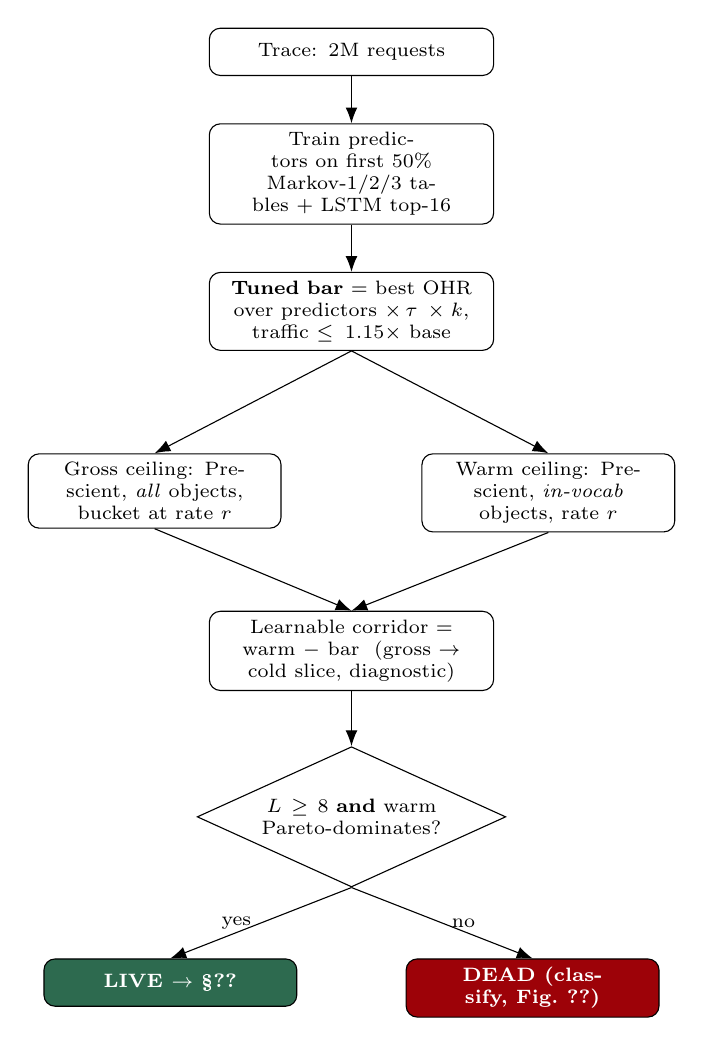
\begin{tikzpicture}[
  node distance=6mm and 6mm,
  box/.style={draw,rounded corners,align=center,font=\scriptsize,inner sep=3pt,minimum height=6mm,text width=3.4cm},
  dia/.style={draw,diamond,aspect=2.2,align=center,font=\scriptsize,inner sep=1pt,text width=2.7cm},
  term/.style={draw,rounded corners,align=center,font=\scriptsize\bfseries,inner sep=3pt,minimum height=6mm,text width=3.0cm},
  ar/.style={-{Latex[length=2mm]}}
]
\node[box] (trace) {Trace: 2M requests};
\node[box,below=of trace] (train) {Train predictors on first 50\%\\ Markov-1/2/3 tables $+$ LSTM top-16};
\node[box,below=of train] (bar) {\textbf{Tuned bar} $=$ best OHR over predictors $\times\,\tau\,\times k$, \ traffic $\leq 1.15\times$ base};
\node[box,text width=3.0cm,below=13mm of bar,xshift=-2.5cm] (gross) {Gross ceiling: Prescient, \emph{all} objects, bucket at rate $r$};
\node[box,text width=3.0cm,below=13mm of bar,xshift=2.5cm] (warm) {Warm ceiling: Prescient, \emph{in-vocab} objects, rate $r$};
\node[box,below=33mm of bar] (learn) {Learnable corridor $=$ warm $-$ bar \ (gross $\to$ cold slice, diagnostic)};
\node[dia,below=7mm of learn] (v) {$L\geq8$ \textbf{and} warm Pareto-dominates?};
\node[term,fill=live,text=white,below=9mm of v,xshift=-2.3cm] (yes) {LIVE $\to$ \S\ref{sec:ladder}};
\node[term,fill=dead,text=white,below=9mm of v,xshift=2.3cm] (no) {DEAD (classify, Fig.~\ref{fig:mech})};
\draw[ar] (trace)--(train);
\draw[ar] (train)--(bar);
\draw[ar] (bar.south)-- (gross.north);
\draw[ar] (bar.south)-- (warm.north);
\draw[ar] (gross.south)--(learn.north);
\draw[ar] (warm.south)--(learn.north);
\draw[ar] (learn)--(v);
\draw[ar] (v.south)-- node[left,font=\scriptsize]{yes} (yes.north);
\draw[ar] (v.south)-- node[right,font=\scriptsize]{no} (no.north);
\end{tikzpicture}
\caption{\textbf{The instrument.} Invariants checked on every run: the bar's and the warm ceiling's cold-prefetch-hit counts are both exactly zero (a history-based predictor's candidates are drawn from its training vocabulary by construction; the warm ceiling is restricted to it by definition). ``base'' $=$ S3-FIFO with no prefetch; its origin bytes are the traffic denominator; $r$ is the bar's measured prefetch byte rate.}
\label{fig:instrument}
\end{figure}

\begin{itemize}\itemsep0.1em
\item \textbf{BASE}: S3-FIFO, no prefetch. Its origin bytes are the traffic denominator for every arm.
\item \textbf{TUNED BAR}: the best decoupled system constructible against the corridor's own interest: max OHR over \{Markov-1, Markov-2, Markov-3 ($3{\to}2{\to}1$ backoff), LSTM\} $\times\ \tau \in \{0.01\ldots0.5\}$ (including 0.06--0.09) $\times\ k \in \{1,2,4\}$, subject to origin traffic $\leq 1.15\times$ BASE. The cap is 1.15, not 1.10, because the default config lands at $1.10\times$ exactly and a 1.10 cap could reject it on float noise; the cap errs \emph{against the corridor} by letting the baseline tune up. The LSTM arm (embedding 128, hidden 256, trained on the prefix, per-position top-16 dumped in one causal GPU pass) exists so the bar is not merely ``best counting table.''
\item \textbf{GROSS CEILING}: Prescient (prefetch the soonest-future uncached objects, $k{=}4$) throttled by a token bucket to the \emph{bar's measured prefetch byte rate}. A rate, not a total budget: a total is spent greedily at trace start and then prefetching stops, which once made an oracle score below a heuristic, the impossible result that exposed the bug. Reported as a diagnostic only.
\item \textbf{WARM CEILING} (primary): Prescient restricted to training-vocab objects, same token bucket. Because the bucket is unchanged, budget the gross oracle spends on unreachable cold objects is \emph{re-spent} on warm ones. This is the honest upper bound for any history-based scheduler: perfect timing, realistic knowledge, equal budget.
\end{itemize}

\subsection{Why the warm ceiling, not subtraction}\label{sec:whywarm}
The tempting shortcut, learnable $\approx$ gross corridor $-$ cold slice, is wrong in both directions. It over-penalizes because the oracle's cold prefetches consumed budget a warm-only policy would redirect (on Wikipedia, 27\% of the gross oracle's useful prefetches were cold; redirected, that budget buys $+5.4$ points of warm hits). It can also under-penalize via eviction coupling (on \texttt{meta\_rprn} the warm ceiling lands 0.35 points \emph{below} the subtraction estimate). Measured on these traces, subtraction misstates the learnable corridor by up to 5.4 points, enough to flip a verdict in either direction. Reachability must be priced \emph{inside} the replay, at the budget, not adjusted afterward on paper.

For provenance: the first cold definition used in this project (``object not yet requested at issue time'') was wrong. A frozen predictor legitimately prefetches an object \emph{ahead} of its first local occurrence if training taught the association. The invariant caught it: the bar showed 442{,}188 ``cold'' hits on Wikipedia where the correct number, under the out-of-vocabulary definition, is zero. Definitions of learnability need machine-checkable invariants precisely because they are where motivated reasoning hides.

\subsection{Escalation protocol and pre-registration}
The verdict bar (learnable corridor $\geq 8$ OHR points \textbf{and} Pareto dominance at the warm ceiling) was fixed before any real-trace run. Baselines escalate in pre-registered stages (coarse Markov-1/2 grid, then fine-$\tau$ plus Markov-3, then LSTM) and \textbf{a LIVE verdict is provisional until it survives the strongest stage}. Two traces that passed early stages were killed by later ones (\S\ref{sec:audit}). The escalation only ever raises the bar, so survival is meaningful and death is final.

\section{Results: Measurement}\label{sec:results}
\subsection{Gross corridors and their deaths}
\begin{table*}[t]\centering\footnotesize
\setlength{\tabcolsep}{4pt}
\caption{Gate A across 12 traces (gross corridor $=$ gross ceiling $-$ tuned bar, iso-BW; strongest-bar values where escalation ran).}
\label{tab:gatea}
\begin{tabular}{llccccp{4.3cm}}
\toprule
trace & family & base OHR & tuned bar & gross corr. & gross verdict & kill mechanism \\
\midrule
\texttt{wiki\_2019t} & CDN & 0.152 & 0.5531 @1.09\x & $+26.49$ & live $\to$\S\ref{sec:learnable} & (none) \\
\texttt{meta\_rprn} & CDN & 0.390 & 0.6738 @1.03\x & $+32.57$ & live $\to$\S\ref{sec:learnable} & cold-dominated \\
\texttt{meta\_reag} & CDN & 0.538 & 0.7547 @1.11\x & $+24.51$ & live $\to$\S\ref{sec:learnable} & cold-dominated \\
\texttt{cluster50} & KV & 0.416 & 0.7080 @1.02\x & $+20.37$ & live $\to$\S\ref{sec:learnable} & (none) \\
\texttt{cluster53} & KV & 0.595 & 0.6101 @1.10\x (LSTM) & $+25.72$ & live $\to$\S\ref{sec:learnable} & (none) \\
\texttt{cluster26} & KV & 0.786 & 0.8907 @1.09\x & $+10.27$ & \textbf{DEAD} & traffic-bought (ceiling $1.16\times$ vs bar $1.09\times$) \\
\texttt{cluster10} & KV & 0.500 & 0.7368 @1.00\x & $-1.18$ & DEAD & degenerate predictability (precision 1.000; bar $>$ ceiling) \\
\texttt{msr\_proj\_0} & block & 0.552 & 0.7568 @1.13\x & $+4.16$ & DEAD & bar saturation (robust to any cap: $+3.7$ to $+5.5$) \\
\texttt{msr\_hm\_0} & block & 0.657 & 0.8380 @1.13\x & $+10.08$ & live $\to$\S\ref{sec:learnable} & cold $+$ saturation \\
\texttt{msr\_web\_2} & block & 0.010 & 0.8284 @1.00\x & $-3.81$ & DEAD & bar saturation (precision 0.996 @1.00\x) \\
\texttt{w105} & block & 0.269 & 0.8494 @1.05\x & $-0.45$ & DEAD & bar saturation \\
\texttt{w87} & block & 0.095 & 0.5383 @1.12\x & $+32.67$ & DEAD$^{*}$ & Pareto fail by $0.01\times$; boundary, cited neither way \\
\bottomrule
\end{tabular}
\end{table*}

Table~\ref{tab:gatea} makes three points. First, the tuned bar is doing real work: on \texttt{cluster26} the escalation from a coarse Markov-1/2 grid to fine-$\tau$ plus Markov-3 raised the bar five points ($0.841{\to}0.891$) and flipped a provisional LIVE to DEAD. Second, the LSTM arm took the bar exactly once (\texttt{cluster53}), left it untouched everywhere else, and never rescued a corridor: the corridors that survive are not weak-predictor artifacts. Third, liveness is not a family property: MSR block traces produce both $+10.08$ and $-3.81$; Twitter KV produces both $+25.72$ and $-1.18$.

\subsection{The learnable corridor: 14--87\% of the gross is phantom}\label{sec:learnable}
\begin{table}[t]\centering\footnotesize
\setlength{\tabcolsep}{4pt}
\caption{Warm/cold decomposition on the six gross-live traces (all runs verify bar-cold $=0$ and warm-cold $=0$).}
\label{tab:learnable}
\begin{tabular}{lccccl}
\toprule
trace & gross & cold (pts) & warm ceil. & \textbf{learnable} & verdict \\
\midrule
\texttt{cluster53} & $+24.46$ & 4.62 & 0.7940 & $\mathbf{+19.67}^{\dagger}$ & \textbf{LIVE} \\
\texttt{cluster50} & $+20.37$ & 2.69 & 0.8836 & $\mathbf{+17.56}$ & \textbf{LIVE} \\
\texttt{wiki\_2019t} & $+26.49$ & 19.22 & 0.6803 & $\mathbf{+12.72}$ & \textbf{LIVE} \\
\texttt{msr\_hm\_0} & $+10.08$ & 5.82 & 0.8869 & $+4.89$ & dead \\
\texttt{meta\_rprn} & $+32.57$ & 27.90 & 0.7169 & $+4.32$ & dead \\
\texttt{meta\_reag} & $+24.55$ & 20.71 & 0.7906 & $+3.63$ & dead \\
\bottomrule
\end{tabular}
\end{table}

\begin{figure}[t]
\centering
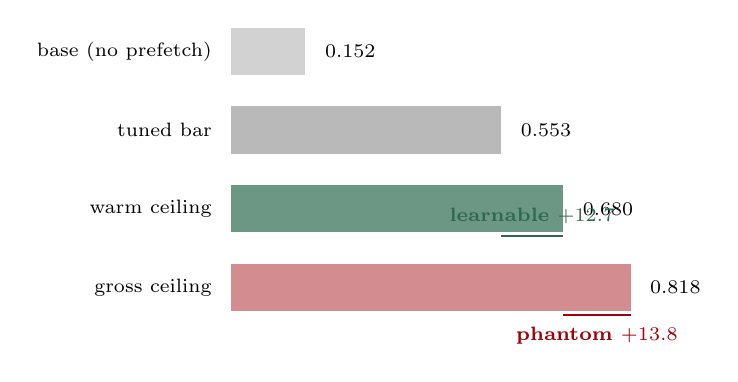
\begin{tikzpicture}[x=6.2cm,y=1cm]
\foreach \v/\yy/\lab/\col in {
  0.152/3/{base (no prefetch)}/gray!35,
  0.553/2/{tuned bar}/gray!55,
  0.680/1/{warm ceiling}/live!70,
  0.818/0/{gross ceiling}/dead!45}{
  \fill[\col] (0,\yy) rectangle (\v,\yy+0.6);
  \node[anchor=west,font=\scriptsize] at (\v+0.02,\yy+0.3) {\v};
  \node[anchor=east,font=\scriptsize] at (-0.02,\yy+0.3) {\lab};
}
\draw[thick,live] (0.553,0.95) -- (0.680,0.95);
\node[font=\scriptsize\bfseries,live,anchor=south] at (0.616,0.98) {learnable $+12.7$};
\draw[thick,dead] (0.680,-0.05) -- (0.818,-0.05);
\node[font=\scriptsize\bfseries,dead,anchor=north] at (0.749,-0.08) {phantom $+13.8$};
\end{tikzpicture}
\caption{\textbf{Corridor anatomy, Wikipedia} (all arms at iso-bandwidth, OHR). The gross corridor ($+26.5$) that a headline evaluation would report decomposes into $+12.7$ reachable by a perfectly-timed history-based policy and $+13.8$ (52\%) reachable only by clairvoyance.}
\label{fig:anatomy}
\end{figure}

The deflation is workload-dependent in a mechanistic way: the three CDN/block traces with the most impressive gross corridors ($+24.5$ to $+32.6$) lose 51--87\% of them to the cold slice, because high object churn means the clairvoyant ceiling spends its budget eliminating compulsory misses. The two low-churn KV traces lose only 14--20\%. Wikipedia is the instructive middle case: high churn (52\% phantom) \emph{and} enough exploitable warm reuse that the honest corridor still clears the bar, but only once the warm ceiling re-spends the cold budget (naive subtraction leaves it at $+7.27$, a false kill).

\subsection{Are the survivors solid? Paired block-bootstrap CIs}
Per-request hit indicators for bar and warm ceiling are recorded on the same post-warmup requests; the corridor is the mean of the paired difference, resampled as 1{,}000 contiguous blocks with replacement, 10{,}000 resamples (block, not i.i.d., because hit outcomes are temporally autocorrelated through cache state).

\begin{table}[h]\centering\footnotesize
\caption{Learnable corridor, 95\% CIs. Pre-registered rule: reliably live only if the CI lower bound $\geq 8$.}
\label{tab:boot}
\begin{tabular}{lcccc}
\toprule
trace & learnable & 95\% CI & SE & verdict \\
\midrule
\texttt{cluster53} & $+19.67$ & $[+19.41,+19.93]$ & 0.13 & reliably LIVE \\
\texttt{cluster50} & $+17.56$ & $[+15.78,+19.39]$ & 0.93 & reliably LIVE \\
\texttt{wiki\_2019t} & $+12.72$ & $[+10.93,+14.52]$ & 0.92 & reliably LIVE \\
\bottomrule
\end{tabular}
\end{table}

All three lower bounds clear the bar; Wikipedia, the lowest-margin trace, retains $\approx3$ points of slack at its 2.5th percentile. ($^{\dagger}$\texttt{cluster53}'s decomposition and CI use its Markov bar (0.5973 @1.01\x); the LSTM bar is 1.28 pts higher at a larger budget. Against the LSTM bar, with the warm ceiling still handicapped to the smaller Markov budget, the corridor is $\geq +18.4$; the verdict is unchanged under the conservative reading.)

\subsection{The instrument versus its authors: an audit trail}\label{sec:audit}
A protocol's credibility is what it catches, including from its own authors. In chronological order, on the record:
\begin{enumerate}\itemsep0.1em
\item \textbf{The $+42$ that became $-0.02$} (synthetic): the first corridor used a default-config baseline and an oracle with unmatched bandwidth. Tuning the bar and matching bytes erased it entirely.
\item \textbf{The $+12.48$ that became DEAD} (\texttt{cluster26}): a coarse $\tau$ grid hid cap-edge configurations; the fine grid plus Markov-3 raised the bar five points, and the Pareto check showed even clairvoyance buys the residual corridor with 7\% extra traffic.
\item \textbf{A retracted cold definition}: the first ``cold'' (never-yet-requested at issue) violated its own invariant; the \emph{bar} scored 442k cold hits where the correct count is zero. The out-of-vocabulary definition restored the invariant.
\item \textbf{A false kill reversed for a principled reason} (Wikipedia): under naive subtraction wiki fell to $+7.27$, below the bar. The warm ceiling, adopted because subtraction is \emph{wrong}, not because the verdict displeased, measures $+12.72$. The 8-point bar never moved in either direction.
\end{enumerate}
Part II extends this trail: the capture gates below caught five further arm bugs before any of them reached a conclusion, including two in the gates' own oracle arms (\S\ref{sec:f7}, \S\ref{sec:llm}). A gate that never catches anything is not a gate.

\begin{figure}[t]
\centering
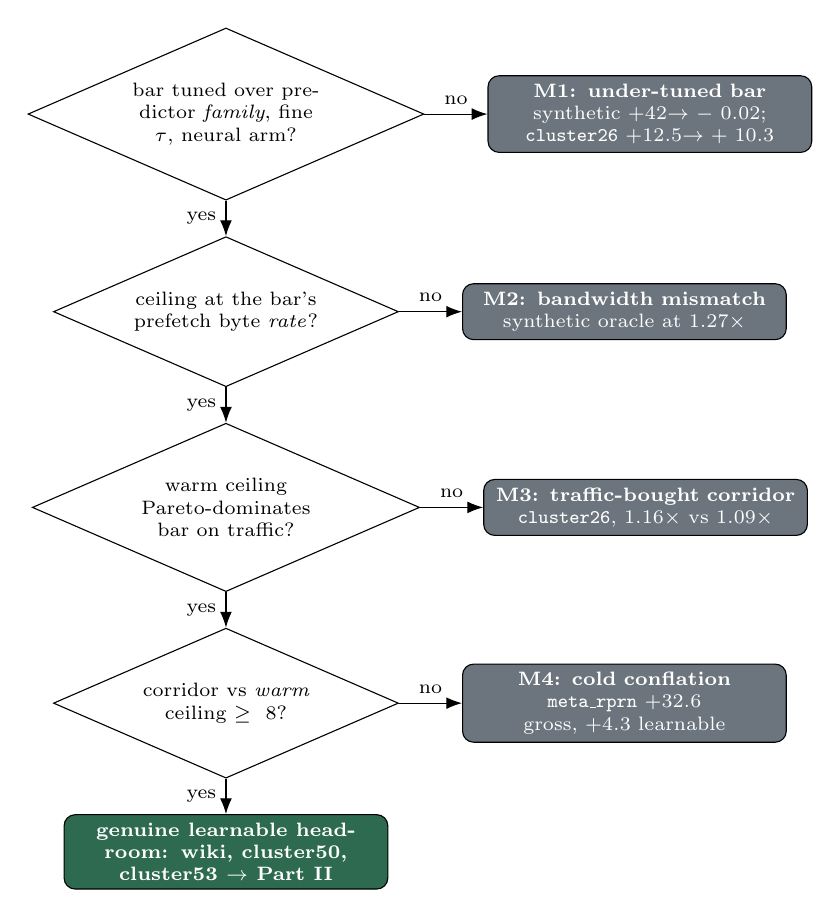
\begin{tikzpicture}[
  node distance=4.5mm and 8mm,
  dia/.style={draw,diamond,aspect=2.3,align=center,font=\scriptsize,inner sep=1pt,text width=3.0cm},
  kill/.style={draw,rounded corners,fill=killc,text=white,align=center,font=\scriptsize,inner sep=3pt,text width=3.9cm},
  ok/.style={draw,rounded corners,fill=live,text=white,align=center,font=\scriptsize\bfseries,inner sep=3pt,text width=3.9cm},
  ar/.style={-{Latex[length=2mm]}}
]
\node[dia] (q1) {bar tuned over predictor \emph{family}, fine $\tau$, neural arm?};
\node[kill,right=of q1] (k1) {\textbf{M1: under-tuned bar}\\ synthetic $+42{\to}-0.02$; \texttt{cluster26} $+12.5{\to}+10.3$};
\node[dia,below=of q1] (q2) {ceiling at the bar's prefetch byte \emph{rate}?};
\node[kill,right=of q2] (k2) {\textbf{M2: bandwidth mismatch}\\ synthetic oracle at $1.27\times$};
\node[dia,below=of q2] (q3) {warm ceiling Pareto-dominates bar on traffic?};
\node[kill,right=of q3] (k3) {\textbf{M3: traffic-bought corridor}\\ \texttt{cluster26}, $1.16\times$ vs $1.09\times$};
\node[dia,below=of q3] (q4) {corridor vs \emph{warm} ceiling $\geq 8$?};
\node[kill,right=of q4] (k4) {\textbf{M4: cold conflation}\\ \texttt{meta\_rprn} $+32.6$ gross, $+4.3$ learnable};
\node[ok,below=of q4] (ok) {genuine learnable headroom: wiki, cluster50, cluster53 $\to$ Part II};
\draw[ar] (q1)-- node[above,font=\scriptsize]{no} (k1);
\draw[ar] (q2)-- node[above,font=\scriptsize]{no} (k2);
\draw[ar] (q3)-- node[above,font=\scriptsize]{no} (k3);
\draw[ar] (q4)-- node[above,font=\scriptsize]{no} (k4);
\draw[ar] (q1)-- node[left,font=\scriptsize]{yes} (q2);
\draw[ar] (q2)-- node[left,font=\scriptsize]{yes} (q3);
\draw[ar] (q3)-- node[left,font=\scriptsize]{yes} (q4);
\draw[ar] (q4)-- node[left,font=\scriptsize]{yes} (ok);
\end{tikzpicture}
\caption{\textbf{Four corridor-inflation mechanisms}, each with the component that catches it and the trace that exhibits it.}
\label{fig:mech}
\end{figure}

\section{Mechanism: what separates live from dead}\label{sec:mechanism}
The dead traces are not ``hard'' and the live ones ``easy''; the separation is a two-factor property visible in Table~\ref{tab:learnable}'s bar-vs-warm-ceiling gaps:
\begin{itemize}\itemsep0.1em
\item \textbf{Dead: the tuned bar already saturates the warm ceiling.} \texttt{meta\_reag} (bar 0.754 vs warm 0.791), \texttt{msr\_hm\_0} (0.838 vs 0.887), \texttt{meta\_rprn} (0.674 vs 0.717): whatever warm reuse exists, a well-swept counting table already times it. What remains of the gross corridor is compulsory cold, unreachable by construction.
\item \textbf{Live: exploitable warm reuse the tuned predictor fails to convert.} Wikipedia's bar (0.553) sits 12.7 points under its warm ceiling (0.680): the reuse is in-vocabulary and perfectly-servable at the same budget, but fixed-threshold association prefetching cannot schedule it. Same shape on \texttt{cluster50} (0.708 vs 0.884) and \texttt{cluster53}.
\end{itemize}
The learnable corridor is therefore exactly the quantity a learned prefetch scheduler should target, and the natural next act of a systems paper would be to build one. Part II explains why that would fail, and proves it with oracles instead of a trained model's ambiguous defeat.

\section{Eviction and prefetching are substitutes ($n{=}6$)}\label{sec:substitutes}
If better eviction and better prefetching fixed \emph{different} misses, a joint policy could exploit the coupling. The interaction is measured directly: a $2\times2$ of \{S3-FIFO, Belady\} $\times$ \{no prefetch, Prescient@matched-BW\} per trace; the interaction is (eviction gain under oracle prefetch) $-$ (eviction gain without prefetch). Six traces: \texttt{msr\_proj\_0} $-1.34$, \texttt{msr\_hm\_0} $-2.31$, wiki $-3.88$, \texttt{cluster53} $-6.66$, \texttt{cluster50} $-7.83$, \texttt{meta\_rprn} $-7.94$. \textbf{All negative: substitutes.} Better prefetching shrinks what better eviction can add on every trace measured; they compete for the same misses. (On variable-size CDN/KV objects Belady is a strong heuristic, not a proven optimum~\cite{demandmin}; only the uniform-block MSR rows carry ``optimal'' strictly.)

Two implications. For system design: joint eviction-plus-prefetch co-training chases a coupling that is negative everywhere measured; the decoupled architecture (strong fixed evictor plus separate prefetch scheduling) is not a simplification but the indicated design, and it licenses freezing S3-FIFO in every capture experiment below. For this project's history: this result killed the joint-RL thesis the project began with, and it is reported as a finding rather than repurposed as motivation.

\section{Part II: The Necessity Ladder}\label{sec:ladder}
The three live corridors invite an obvious system: a learned scheduler that captures them. The Necessity Ladder replaces that reflex with a question sequence, each rung a pre-registered, replay-only gate that isolates \emph{one} ingredient of the hypothetical system with an oracle and prices it before anything is trained. A rung must clear its gate to justify paying for the next; a failed gate is a finding, not a setback. Figure~\ref{fig:ladder} shows the ladder as run; Table~\ref{tab:decomp} collects the decomposition it produces. Every arm below keeps S3-FIFO frozen, respects the bar's byte budget through the same token bucket, and reports paired block-bootstrap CIs. Oracle arms exist only to bound what is possible; none is ever reported as an achievable result.

\begin{figure}[t]
\centering
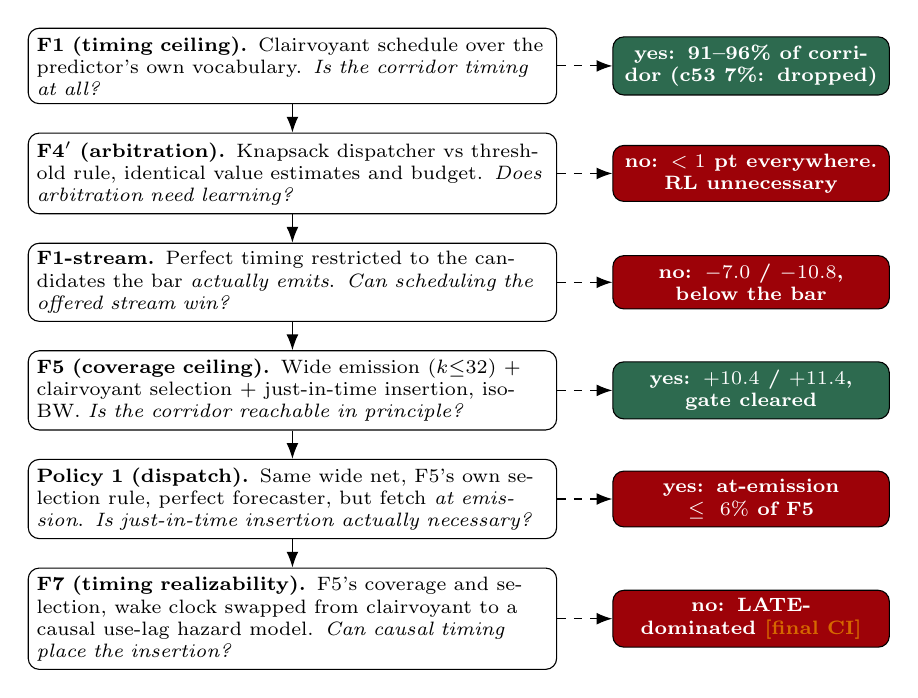
\begin{tikzpicture}[
  node distance=3.6mm and 7mm,
  rung/.style={draw,rounded corners,align=left,font=\scriptsize,inner sep=3pt,text width=6.5cm},
  verd/.style={draw,rounded corners,align=center,font=\scriptsize\bfseries,inner sep=3pt,text width=3.3cm},
  ar/.style={-{Latex[length=2mm]}}
]
\node[rung] (f1) {\textbf{F1 (timing ceiling).} Clairvoyant schedule over the predictor's own vocabulary. \emph{Is the corridor timing at all?}};
\node[verd,fill=live,text=white,right=of f1] (v1) {yes: 91--96\% of corridor (c53 7\%: dropped)};
\node[rung,below=of f1] (f4) {\textbf{F4$'$ (arbitration).} Knapsack dispatcher vs threshold rule, identical value estimates and budget. \emph{Does arbitration need learning?}};
\node[verd,fill=dead,text=white,right=of f4] (v4) {no: $<1$ pt everywhere. RL unnecessary};
\node[rung,below=of f4] (fs) {\textbf{F1-stream.} Perfect timing restricted to the candidates the bar \emph{actually emits}. \emph{Can scheduling the offered stream win?}};
\node[verd,fill=dead,text=white,right=of fs] (vs) {no: $-7.0$ / $-10.8$, below the bar};
\node[rung,below=of fs] (f5) {\textbf{F5 (coverage ceiling).} Wide emission ($k{\leq}32$) $+$ clairvoyant selection $+$ just-in-time insertion, iso-BW. \emph{Is the corridor reachable in principle?}};
\node[verd,fill=live,text=white,right=of f5] (v5) {yes: $+10.4$ / $+11.4$, gate cleared};
\node[rung,below=of f5] (p1) {\textbf{Policy 1 (dispatch).} Same wide net, F5's own selection rule, perfect forecaster, but fetch \emph{at emission}. \emph{Is just-in-time insertion actually necessary?}};
\node[verd,fill=dead,text=white,right=of p1] (vp) {yes: at-emission $\leq6\%$ of F5};
\node[rung,below=of p1] (f7) {\textbf{F7 (timing realizability).} F5's coverage and selection, wake clock swapped from clairvoyant to a causal use-lag hazard model. \emph{Can causal timing place the insertion?}};
\node[verd,fill=dead,text=white,right=of f7] (v7) {no: LATE-dominated \pend{final CI}};
\draw[ar] (f1)--(f4); \draw[ar] (f4)--(fs); \draw[ar] (fs)--(f5); \draw[ar] (f5)--(p1); \draw[ar] (p1)--(f7);
\draw[ar,dashed] (f1.east)--(v1.west); \draw[ar,dashed] (f4.east)--(v4.west); \draw[ar,dashed] (fs.east)--(vs.west);
\draw[ar,dashed] (f5.east)--(v5.west); \draw[ar,dashed] (p1.east)--(vp.west); \draw[ar,dashed] (f7.east)--(v7.west);
\end{tikzpicture}
\caption{\textbf{The Necessity Ladder as run.} Each rung is a pre-registered oracle decomposition isolating one ingredient; the corridor survives every rung that could certify it and dies on the only ingredient no causal policy can supply.}
\label{fig:ladder}
\end{figure}

\subsection{F1: the corridor is timing, in principle}\label{sec:f1}
F1 keeps the predictor's candidate universe fixed and replaces only issue timing with an oracle: a clairvoyant schedule over the objects the predictor could ever name, at the bar's byte rate. On Wikipedia F1 recovers 95.8\% of the learnable corridor and on \texttt{cluster50} 91.2\%: the corridor is almost entirely a scheduling quantity, not an object-choice quantity. On \texttt{cluster53} F1 recovers only 7.3\%, so that trace leaves the capture study here (its corridor is object choice, a predictor problem); the capture claims below are evaluated on both remaining live traces, never on one.

\subsection{F4$'$: learned arbitration is unnecessary}\label{sec:f4}
Before any reinforcement learner earns a training budget, its decision problem must be shown to be non-separable: a joint chooser must beat a per-candidate threshold rule given identical value estimates and an identical byte budget. Two arms differ only in the funding rule (separable: fund by value-per-byte threshold; joint: value-maximizing knapsack over the pending pool with bounded swap improvement). A clairvoyant control (both arms given true values) reads $\approx0$ as expected, validating the solver. With the predictor's own confidences, the gap is $+0.01$ points on Wikipedia and $-0.01$ on \texttt{cluster50}. The pre-registered gate (RL earns a budget only if the gap exceeds 2 points) fails by two orders of magnitude. Prefetch arbitration at this granularity is separable; a threshold rule is the method.

\subsection{F1-stream: perfect timing of what is offered loses}\label{sec:f1stream}
F1's vocabulary oracle could still choose \emph{which} in-vocabulary objects to fetch. F1-stream removes that freedom: perfect timing, applied only to the candidate stream the tuned bar actually emits ($k{=}1$ per request), dropping candidates never used again (precision 1.0). It lands \emph{below} the bar on both traces: $-7.01$ $[-7.68,-6.33]$ on Wikipedia, $-10.82$ $[-11.70,-9.93]$ on \texttt{cluster50}. No scheduler, however clever, can beat the baseline by re-timing the candidates the baseline already names: the predictor names each object too rarely for anything to schedule. The corridor is a \emph{coverage} problem.

\subsection{F5: coverage plus clairvoyant timing reaches the corridor}\label{sec:f5}
F5 widens the emission net (fanout $k$ up to 32, confidence floor removed) and defines a use as \emph{causally coverable} if the wide predictor emitted the object since its previous use; a clairvoyant scheduler then covers only coverable uses, just in time, at the bar's byte rate. Coverage climbs with fanout (Wikipedia 53.6\% at $k{=}1$ to 74.1\% at $k{=}32$), and the ceiling clears the pre-registered gate on both traces: $+10.41$ $[+8.74,+12.08]$ on Wikipedia ($k{=}32$), $+11.42$ $[+9.95,+12.91]$ on \texttt{cluster50} ($k{=}16$). The corridor is reachable in principle: width supplies the candidates, and perfectly timed insertion converts them. Two ingredients remain to make this causal: the dispatch rule and the timing.

\subsection{Policy 1: at-emission dispatch captures $\leq$6\%, even with a perfect forecaster}\label{sec:policy1}
The causal realization of F5 fetches candidates when they are emitted and holds them until use. To separate the dispatch design from forecaster quality, the diagnostic arm uses a \emph{perfect} forecaster ranked by F5's own selection rule (soonest use first), so the only difference from F5 is \emph{when} the fetch happens: at emission rather than just in time. The result, in every configuration on both traces, is a loss of 10--15 points to F5; at-emission dispatch captures at most 6\% of the F5 corridor (Wikipedia, best case), and is negative on \texttt{cluster50}. Since even a perfect forecaster fails at emission, no better-trained forecaster can rescue this design: the missing ingredient is isolated, cleanly, as just-in-time insertion. (A fairness control accompanies every rate-limited comparison: the bar re-run under the same token bucket the scheduler faces, so protocol cost is never misread as scheduling failure; this control reappears in \S\ref{sec:llm}.)

\subsection{F7: causal timing cannot place the insertion}\label{sec:f7}
One ingredient remains. F7 keeps F5's clairvoyant coverage and selection (every funded object will be used again; the \emph{what} is guaranteed) and swaps only the wake clock: \texttt{oracle} (true next use, the construction check), versus \texttt{model} (a causal hazard model of time-to-next-use, binned over recency, frequency, and confidence, trained on a held-out window with a three-way split), versus a median-only diagnostic. The pre-registered gate: the model arm captures at least 50\% of the oracle arm's corridor, CI clear of zero, swept over the hedging quantile $\gamma$.

The hazard model \emph{passes} the standard learnability gate that would normally justify building on it: Spearman rank correlation between predicted and true lags of $+0.60$ (Wikipedia) and $+0.43$ (\texttt{cluster50}), never-used AUC 0.92 and 0.81. The construction check passes: the oracle arm reproduces the F5 ceiling (102.4\% of F5 on \texttt{cluster50}, $+11.69$ $[+10.23,+13.18]$, 100\% on-time). The model arm nevertheless fails catastrophically: at the most forgiving quantile ($\gamma{=}0.1$, earliest wake), fetches land LATE (after the use, a total loss) on 74--93\% of insertions through the first half of both traces, and higher quantiles are monotonically worse. \pend{Final model-arm capture and CI, both traces, primary and wide-retrained-hazard fallback: runs completing; the pre-registered fallback retrains the hazard model on the wide emission stream before the kill is accepted.} Instrumentation added for honesty separates two failure modes within LATE: genuine forecast overshoot (the predicted wake lands after the use) and bandwidth queuing (the wake was early but the bar-sized token bucket funds the fetch after the use). Both are substantial; the claim the number supports is therefore precise: \emph{causal just-in-time warming under the baseline's bandwidth budget is unreachable}, which is the deployable question.

\begin{table}[t]\centering\footnotesize
\setlength{\tabcolsep}{4pt}
\caption{The capture decomposition: which combination of ingredients reaches the corridor. Oracle ingredients in \textcolor{dead}{red} are unavailable to any deployable policy; the only all-causal row is bounded above by every failed mixed row.}
\label{tab:decomp}
\begin{tabular}{llllc}
\toprule
selection (\emph{what}) & insertion (\emph{when}) & arm & wiki & cluster50 \\
\midrule
\textcolor{dead}{clairvoyant, wide} & \textcolor{dead}{clairvoyant JIT} & F5 & $+10.41$ & $+11.42$ \\
causal, $k{=}1$ stream & \textcolor{dead}{clairvoyant JIT} & F1-stream & $-7.01$ & $-10.82$ \\
\textcolor{dead}{clairvoyant, wide} & at emission & Policy 1 & $\leq+0.62$ & $<0$ \\
\textcolor{dead}{clairvoyant, wide} & causal hazard & F7 model & \pend{pending} & \pend{pending} \\
causal & causal & any deployable & \multicolumn{2}{c}{$\leq$ min of rows above} \\
\bottomrule
\end{tabular}
\end{table}

\subsection{The mechanism: endogenous slack}\label{sec:slack}
Why does a hazard model that ranks lags well ($\rho\approx0.6$) fail so completely at placement? The answer is a feedback loop the gates expose directly. Under the \emph{bar's} modest fetch load, prefetched objects essentially never leave the cache before use ($S(100){=}1.0$: survival past 100 requests is certain), so a timing model would seem to enjoy enormous slack. But slack is not a property of the workload; it is a property of the policy's own behavior. A wide-net causal policy that mistimes fetches issues far more of them (precision collapses toward 0.05), and that volume churns the cache, which collapses the survival curve, which shrinks the residence window every subsequent fetch must hit, which makes mistiming more costly still. Clairvoyant insertion needs zero slack (arrive one request early); a log-binned hazard model has multiplicative error on heavy-tailed lag distributions, so at any hedging quantile it simultaneously overshoots some uses (LATE) and arrives so early on others that its own churn evicts the object before use. The two failure modes pincer the policy at every $\gamma$.

The general lesson: \textbf{rank-learnable is not placeable}. A learnability gate certifies that a signal orders correctly; an insertion decision needs the signal to land inside a window whose width the decision itself determines. Headroom studies and learned-prefetcher evaluations do not currently distinguish these, and the F2-pass/F7-fail pair measured here is, to current knowledge, the first direct demonstration that the gap between them can be total.

\section{Part III: the ruler discriminates, LLM KV-cache serving}\label{sec:llm}
A measurement instrument earns trust by returning \emph{different} answers on different inputs. The instrument was therefore ported to a second, economically pressing domain: KV-cache warming in LLM serving, on the production traces released by Mooncake~\cite{mooncake} (one hour each of conversation and tool/agent traffic from a large deployed platform; objects are 512-token KV blocks with hashed identities, so identical IDs mark reusable prefixes). Warming a block into the HBM cache before its next use is the prefetch analog; OHR measures prefill compute avoided, the time-to-first-token lever.

Two adaptations keep the port honest rather than mechanical. First, \emph{turn gating}: a request's blocks are read simultaneously at prefill, so per-access prefetching inside an in-flight request would fake-convert whole prefix chains at zero latency. Every arm, bar and ceiling alike, may issue warmings only at request boundaries; the corridor then measures exactly the deployable quantity, cross-turn warming. Second, the reachability restriction becomes \emph{physical}: a KV block never computed and stored cannot be warmed by any system, so the warm ceiling is the true ceiling in this domain, not merely the budget-fair one. The pre-registered fork, fixed before the first run, reuses the paper's bars unchanged (corridor $\geq8$, CI $>0$, Pareto; lag learnability at Spearman $\geq0.20$, AUC $\geq0.60$). A protocol control (the bar re-run under the ceiling's token bucket) separates burst-versus-bucket protocol cost from scheduling quality; without it, the burst-capable bar's advantage would masquerade as a negative corridor.

\begin{table}[t]\centering\footnotesize
\setlength{\tabcolsep}{3.5pt}
\caption{The instrument on Mooncake production traces (1\% block cache, full predictor/threshold/degree sweep, invariants all pass). BAR-CAP is the bar under the ceiling's token bucket; the like-for-like column is ceiling minus BAR-CAP.}
\label{tab:llm}
\begin{tabular}{lcccccc}
\toprule
trace & base & tuned bar & warm ceil. & corridor & 95\% CI & like-for-like \\
\midrule
conversation & 0.079 & \textbf{0.151} & 0.145 & $-0.56$ & $[-1.14,+0.04]$ & $+2.98$ \\
tool/agent & 0.366 & \textbf{0.444} & 0.425 & $-1.87$ & $[-2.38,-1.36]$ & $+2.14$ \\
\bottomrule
\end{tabular}
\end{table}

The verdict (Table~\ref{tab:llm}) is the third distinct outcome the instrument has produced: \textbf{no corridor exists}. A tuned Markov table over block IDs already sits within noise of the physically reachable, bandwidth-matched clairvoyant ceiling on both traces; even under identical protocol the clairvoyant margin is $+2$--$3$ points against an 8-point gate. The reason is visible in the domain's structure: prefix-chain reuse is nearly deterministic (held-out next-request coverage 0.728 for the association table versus 0.008 for a popularity baseline), so the trivial policy is already the ceiling. Notably, the conversation trace's reuse \emph{timing} is learnable (think-time hazard: Spearman $+0.27$, AUC 0.81), but there is no corridor for that signal to capture; the tool/agent trace has neither ($\rho{=}0.003$). Anyone about to train an ML-based KV-cache warmer, a currently fashionable system, would be told by one replay: do not.

\begin{table}[t]\centering\footnotesize
\setlength{\tabcolsep}{4pt}
\caption{Three workload families, three pre-registered verdicts, all reached before training a model.}
\label{tab:threedomains}
\begin{tabular}{lll}
\toprule
domain & verdict & mechanism \\
\midrule
block storage (MSR, CloudPhysics) & corridor absent & bar saturation / cold domination \\
CDN / KV (wiki, Twitter) & corridor present, \textbf{clairvoyance-priced} & endogenous slack kills causal timing \\
LLM KV serving (Mooncake) & corridor absent & tuned table is already the physical ceiling \\
\bottomrule
\end{tabular}
\end{table}

\section{Scope and threats to validity}
\begin{itemize}\itemsep0.1em
\item \textbf{``Learnable'' is defined against frozen, history-based prediction} (training-prefix vocabulary). An online-updating predictor could reach an object from its second occurrence onward; content-aware prediction could reach some cold objects. Both would \emph{raise} live corridors and could revive dead traces; the measurement verdicts are conservative in that direction. The capture verdict is not symmetric: F5's coverage ceiling already grants the widest emission the predictor family supports, and F7's failure is a timing failure that a larger vocabulary does not touch.
\item \textbf{The capture kill is bounded by its oracle decomposition.} The ladder prices the ingredient combinations in Table~\ref{tab:decomp}; a design outside that decomposition (for example, one that modifies the evictor to protect warmed objects) is out of scope, though the substitutes result argues against expecting gains from evictor coupling. The F7 kill is accepted only after the pre-registered fair-shot fallback (retraining the hazard model on the wide emission stream it is evaluated on) \pend{fallback completing}.
\item \textbf{One cache size (1\% of footprint), 2M-request prefixes, request-weighted OHR.} Byte-weighted columns are in the supplement; cache-size sweeps are future work. Twitter traces are 1-in-10 samples (as published), which stretches inter-reference gaps; corridors on sampled traces are internally consistent but absolute OHRs are not comparable to unsampled deployments.
\item \textbf{LLM traces cover one hour of one provider}, and lags are measured in access-index units rather than wall-clock. The screen is evidence about this workload class, not a universal claim; the artifact makes extension to other serving traces a one-command exercise.
\item \textbf{CIs cover within-trace sampling variance only}, not trace choice or sweep granularity. The escalation protocol addresses the latter structurally: every error in the bar inflates corridors, so surviving corridors are lower bounds on scrutiny, and the capture kills are upper bounds on it.
\end{itemize}

\section{Conclusion}
Measured honestly, against a family-tuned baseline, at matched bandwidth, above a ceiling restricted to reachable objects, most celebrated prefetch headroom in caching is phantom: 14--87\% of gross corridors evaporate across 12 production traces, and the biggest corridors lose the most. What survives is real, bootstrap-solid, and concentrated where in-vocabulary reuse exists but fixed-threshold prediction mistimes it. The natural conclusion, build a learned scheduler, is then tested the cheap way: a ladder of pre-registered oracle decompositions prices each ingredient such a system could contribute. Learned arbitration adds under a point. Perfect timing of the offered candidates loses to the baseline. Wide coverage with clairvoyant insertion reaches the corridor, but fetching at prediction time forfeits it even with a perfect forecaster, and the one remaining ingredient, causal insertion timing, fails for a reason with a name: endogenous slack, the policy's own mistimed volume destroying the residence window its timing model must hit. Rank-learnable is not placeable, and the distinction is measured, not conjectured. The corridor that survives the honest ruler is priced in clairvoyance.

The instrument's value is that it discriminates. On block storage it reports no corridor; on CDN and KV traces a corridor that no causal policy can capture; on LLM KV-cache serving, the domain where a learned warmer is currently most tempting, no corridor at all, because a tuned association table already sits on the physical ceiling. Three families, three verdicts, three different mechanisms, each established by replay before a single model was trained, and each a specific answer to the question every learned-systems paper should ask first: is there anything here for learning to win? The gates caught their own authors nine times before they judged anyone else, and that trail, not any single number, is the argument for adopting them. The instrument, the ladder, and all replay code are released so that the next celebrated headroom number can be checked in an afternoon.

\begin{thebibliography}{99}\footnotesize
\bibitem{belady} L.~A. Belady. A study of replacement algorithms for a virtual-storage computer. \emph{IBM Systems Journal} 5(2), 1966.
\bibitem{cao} P.~Cao, E.~W. Felten, A.~R. Karlin, K.~Li. A study of integrated prefetching and caching strategies. \emph{SIGMETRICS}, 1995.
\bibitem{demandmin} A.~Jain, C.~Lin. Rethinking Belady's algorithm to accommodate prefetching (Demand-MIN). \emph{ISCA}, 2018.
\bibitem{lrb} Z.~Song, D.~S. Berger, K.~Li, W.~Lloyd. Learning relaxed Belady for content distribution network caching (LRB). \emph{NSDI}, 2020.
\bibitem{s3fifo} J.~Yang, Y.~Zhang, Z.~Qiu, Y.~Yue, K.~V. Rashmi. FIFO queues are all you need for cache eviction (S3-FIFO). \emph{SOSP}, 2023.
\bibitem{baleen} D.~L.-K. Wong, H.~Wu, C.~Molder, S.~Gunasekar, J.~Lu, S.~Khandkar, A.~Sharma, D.~S. Berger, N.~Beckmann, G.~R. Ganger. Baleen: ML admission \& prefetching for flash caches. \emph{FAST}, 2024.
\bibitem{mooncake} R.~Qin, Z.~Li, W.~He, M.~Zhang, Y.~Wu, W.~Zheng, X.~Xu. Mooncake: A KVCache-centric disaggregated architecture for LLM serving. \emph{FAST}, 2025.
\bibitem{vllm} W.~Kwon, Z.~Li, S.~Zhuang, Y.~Sheng, L.~Zheng, C.~H. Yu, J.~Gonzalez, H.~Zhang, I.~Stoica. Efficient memory management for large language model serving with PagedAttention (vLLM). \emph{SOSP}, 2023.
\bibitem{cachegen} Y.~Liu et al. CacheGen: KV cache compression and streaming for fast large language model serving. \emph{SIGCOMM}, 2024.
\bibitem{coldrl} Cold-RL: Learning cache eviction with offline reinforcement learning for NGINX. arXiv:2508.12485, 2025.
\bibitem{deap} DEAP Cache: Deep eviction admission and prefetching for cache. arXiv:2009.09206, 2020.
\bibitem{deepref} DeePref: Deep reinforcement learning for video prefetching in content delivery networks. arXiv:2310.07881, 2023.
\bibitem{lightcache} LightCacheRL: A lightweight reinforcement learning framework for unified cache management. Springer, 2025. doi:10.1007/978-3-032-10459-5\_11.
\bibitem{pythia} R.~Bera et al. Pythia: A customizable hardware prefetching framework using online reinforcement learning. \emph{MICRO}, 2021.
\bibitem{jointhw} S.~Yuan, D.~Saxena, J.~Chen, N.~Sharma, A.~Akella. A joint learning approach to hardware caching and prefetching. \emph{ML for Systems Workshop @ NeurIPS}, 2025.
\bibitem{sober} A.~Hochlehnert, H.~Bhatnagar, V.~Udandarao, S.~Albanie, A.~Prabhu, M.~Bethge. A sober look at progress in language model reasoning. arXiv:2504.07086, 2025.
\end{thebibliography}

\end{document}
